%!TEX program = <xelatex>
\documentclass[12pt,letterpaper,titlepage]{article}

\usepackage{basicstyle}
\usepackage{notestyle}

\title{
    \vspace{1in}
    \textmd{\textbf{Class Notes for CS6363}}\\
    \textbf{\Large{Design and Analysis of Computer Algorithms}}\\
    \large\vspace{0.1in}\textit{Instructor: Benjamin Raichel}\\
    \vspace{0.1in}\normalsize{University of Texas at Dallas}\\
    Department of Computer Science\\
    \vspace{0.1in}\includegraphics[height=2.4em]{fig/UTD_logo_BW}\\
    \vspace{2in}
}
\author{Hanlin He\\\vspace{0.1in}
\includegraphics[height=4em]{fig/comets_logo_black.pdf}}
\date{}

\makeindex
\begin{document}

\maketitle


\pagenumbering{Roman}
\tableofcontents
\pagebreak
\listofalgorithms
\pagebreak

\pagenumbering{arabic}
\section{Syllabus}
\begin{enumerate}
\item Asymptotic  notation, recurrence.
\item Divide and Conquer.
\item Dynamic Programming.
\item Greedy Algorithm.
\item Graph Algorithm.
\item NPC
\end{enumerate}


\pagebreak

\section{Basic}
\subsection{What is an algorithm?}
Unambiguous, mechanically executable sequence of elementary operations.
There are certain types of algorithm:

\begin{table}[H]
\caption{Comparison between Traditional \& Modern Algorithm}
\centering
\begin{tabular}{ ll }
Traditional (This course’s main focus.) & Modern algorithm research\\
\hline
Deterministic & Randomized \\
Exact & Approximate\\
Off-line & On-line\\
Sequential & Parallel\\
\end{tabular}
\end{table}

\subsection{Input \& Output}

View algorithm as a function with well defined inputs mapping to specific
outputs.

\AlgoInput $A[1...n]$  // Positive real number, distinct.

\AlgoOutput $MAX A[i], 1<= i <= n$.

\subsubsection{Algorithm 1: Stupid way}
\begin{algorithm}[H]
\caption{Stupid Find Max Algorithm}\label{Stupid_Find_Max_Algorithm}
\begin{algorithmic}[1]
\Procedure{FindMax}{}
\For{$i = 1$ to $n$}
  \State $count = 0$
  \For{$j = 1$ to $n$}
    \If{$A[i] > A[j]$}
      \State $count = count + 1$
    \EndIf
  \EndFor
  \If{$count = n$}
    \Return $A[i]$
  \EndIf
\EndFor
\EndProcedure
\end{algorithmic}
\end{algorithm}

\textbf{Analysis}: Worst Case, $n^2$ comparison.

\subsubsection{Algorithm 2: Sort \& Find}
\begin{algorithm}[H]
\caption{Sort \& Find Max Algorithm}\label{Sort_and_Find_Max_Algorithm}
\begin{algorithmic}[1]
\Procedure{FindMax}{}
\State {$\overline{A} = sort(A)$}
\Return $\overline{A}[n]$
\EndProcedure
\end{algorithmic}
\end{algorithm}

\textbf{Analysis}: Worst Case, sorting takes $c\ n\log n$ time.

\subsubsection{Algorithm 3: Dynamically store the biggest one}
\begin{algorithm}[H]
\caption{Search \& Find Max Algorithm}\label{Search_and_Find_Max_Algorithm}
\begin{algorithmic}[1]
\Procedure{FindMax}{}
\State {$current = 1$}
\For{$i = 2$ to $n$}
  \If{$A[i] > A[current]$}
    \State{$current = i$}
  \EndIf
\EndFor
\Return $A[current]$
\EndProcedure
\end{algorithmic}
\end{algorithm}

\subsection{Can we do better?}

It depends on the operations allowed. For example the dropping the curtain and
find the first appearing one.


\pagebreak


\section{Asymptotic Notation -- big ``O'' notation}

\subsection{Growth of Functions}

The growth of function in \cref{function_list} increase downwards.
\begin{table}[H]
\centering
\caption{Function List}\label{function_list}
\begin{tabular}{c|l}
$\log_{10} n$ & binary search \\
$n$ & input \\
$n^2$ & pairs \\
$10^{10}n^{10}$ & \\
$1.000.1^n$ & \\
$2^n$ & Binary string of length n \\
$n!$ & Permutation \\
\end{tabular}
\end{table}
Let $f(n)$, $g(n)$ be function.

\subsection{big ``O'' notation}
\begin{definition}

$f(n) = \bigO{g(n)}$, if $\exists n_0 \in \mathbb{N}$,
$c \in \mathbb{R}^+$, s.t. $\forall n \geq n_0$, $f(n) \leq c * g(n)$,
and $\displaystyle\lim_{n \rightarrow \infty} \frac{f(n)}{g(n)} \ne \infty$,
i.e.\ it is $\displaystyle\lim_{n \rightarrow \infty} \frac{f(n)}{g(n)} < k$, for some constant $k$.
\end{definition}

Table \ref{def_asymptotic_notation} shows the basic definition of all the asymptotic notations.
\begin{table}[H]
\centering
\caption{Definition for all Asymptotic Notation}\label{def_asymptotic_notation}
\begin{tabular}{c|l|c}
\hline
$f(n)$ & $\displaystyle\lim_{n \rightarrow \infty} \frac{f(n)}{g(n)}$ & relation \\
\hline
\hline
$\bigO{g(n)}$ & $\neq \infty$ & $\leq$ \\
$\Omega(g(n))$  & $\neq \infty$ & $\leq$  \\
$\Theta(g(n))$  & $= k > 0$ & $=$  \\
$o(g(n))$  & $= 0$ & $<$  \\
$\omega(g(n))$  & $= \infty$ & $>$  \\
\end{tabular}
\end{table}

\subsection{Asymptotic Relation's feature}
\begin{theorem}
Multiplying by positive constant does NOT change asymptotic relations.
i.e.\ if $f(n) = \bigO{g(n)}$, then $100 * f(n) = \bigO{g(n)}$.
\end{theorem}

\begin{proof}
$f(n) = \bigO{g(n)} \Rightarrow \exists{n_0} \exists c, \forall n \geq n_0, f(n) \leq c*g(n)$,

then, $\exists{n_0}\exists{c'}$, s.t.\ $\forall n \geq n_0$, $100*f(n) \leq c'*g(n) = 100c*g(n)$.
\end{proof}

Example:
\begin{align}
C*2^n & = \Theta(2^n) \\
(C*2)^n & \neq \Theta(2^n)
\end{align}

\begin{claim}
Show: $2n\log(n) - 10n = \Theta(n\log(n))$
\end{claim}

\begin{proof}
First show: $2n\log(n) - 10n = \bigO{n\log(n)}$

For $n_0 = 1$, $c = 2$

\[2n\log(n) - 10n \leq 2n\log(n)\]

Now show: $2n\log(n) - 10n = \Omega(n\log(n))$

For $n_0 = 2^10$, $c = 1$,

\[
\begin{split}
2n\log(n) - 10n & \geq n\log(n) + n \log(2^{10}) - 10n \\
& =n \log(n) + 10n - 10n \\
& =n\log(n) \\
\end{split}
\]

$n_0 = 1$ ($n_0 = 2^{10}$) means $n$ is at least $1$ (or $2^{10}$).
\end{proof}

\begin{corollary}
$\bigO{1}$ means \textbf{Any Constant}.
\end{corollary}

\noindent\textbf{Attention}: \emph{Asymptotic notation has limit. It is not applicable for all scenarios}.

\subsection{Properties of \texorpdfstring{$\log(n)$}{log(n)}}
\definition{$n = C^{\log_c{n}}$, $c > 1$, $\lg{n} = \log_2{n}$, $\ln{n} = \log_e{n}$.}

\begin{corollary}
$\forall{a,b} > 1$

\begin{equation}
\begin{split}
\log_b(n) & = \frac{\log_a(n)}{\log_a(b)} \\
\log_b(n) & = \Theta({\log_a(n)}) \\
\end{split}
\end{equation}

\end{corollary}

\pagebreak
\begin{corollary}
$\forall{a,b} \in \mathbb{R}$

\begin{equation}
\begin{split}
\log(a^n) & = n*\log(a) \\
\log(a*b) & = \log(a) + \log(b)) \\
a^{\log(b)} & = b^{\log(a)} \\
\end{split}
\end{equation}

\end{corollary}

\textup{\textbf{Note}: $\lg(n)$ is to $n$ as n is to $2^n$.}

\subsection{Something More}

\begin{theorem}
Let $f(n)$ be a polynomial function, then $\log(f(n)) = \Theta(\log(n))$.
\end{theorem}

\begin{proof}
    The asymptotic result of $n^2$ and $n^{10}$ are the same.
\end{proof}

\begin{definition}
$\log^*(n) = o(\log\log\log\log\log(n)) = \alpha$.
\end{definition}

Example: $\lg^*(2^{2^{2^{2^{2}}}}) = 5$.


\pagebreak


\section{Series}
\subsection{Some Definition}

\begin{definition}
Harmonic Series:
\[\sum_{i=1}^n {\frac{1}{i}} = \Theta(\log(n))\]
\end{definition}

\begin{definition}
Geometric Series:
\[
\sum_{i=0}^{n-1}{x^i} = \frac{x^n - 1}{x-1} =
\begin{cases}
\Theta(x^n) & \text{if } \forall x>1, \\
\Theta(1) & \text{if } \forall x<1, \\
\Theta(n) & \text{if } \forall x=1.
\end{cases}
\]
\end{definition}

\begin{definition}
Arithmetic Series:
\[\sum_{i=1}^n {i} = \frac{n(n+1)}{2} = \Theta(n^2)\]

\end{definition}

\subsection{Some Theorem}

Suppose I want to know if $f(n) = o(g(n))$.

\begin{theorem}
If $\log(f(n)) = o(\log(g(n))$, then $f(n) = o(g(n))$.
\end{theorem}

Example: Let $f(n) = n^3$, $g(n) = 2^n$. Then $\log(f(n)) = \log(n^3) = 3\log(n)$, $\log(g(n)) = \log(2^n) = n$.
\[\text{i.e. } \log(f(n)) < \log(g(n) \Rightarrow f(n) < g(n)\]

\emph{Note that this theorem stands for `o', NOT TRUE for `$\mathcal{O}$'.}

Example: $\log(n^3) = \mathcal{O}(\log(n^2))$, but $n^3 \neq \mathcal{O}(n^2)$.

\section{Induction}
\subsection{When to use?}
Prove statement for all $n \in \mathbb{N}$, s.t. $n \geq n_0$.

\subsection{Definition}
Basically, induction has two parts:
\begin{enumerate}
\item {Base case(s) -- Sometimes there are more than one base cases.

Prove statement for some $n$. -- Often $n_0 = 0 \text{ or } 1$.}

\item {Induction Hypothesis

Assume statement hold true for all $m \leq n$.

Prove the hypothesis implies that it hold true for $n+1$.}
\end{enumerate}

Note that the process may be different from previous, which just hypothesize $n-1$ is true and prove for $n$.








\pagebreak

\section{Recursion (Divide \& Conquer)}
\begin{itemize}
\item Recursion is like Induction's twin brother, whereas induction is similar to movie filmed, and recursion is similar to movie backward.
\item Recursion design may be most important course topic.
\item Recursion is a type of reduction. \footnote{Reduction is to solve problem A using a black box for B. Typically B is smaller.}
\end{itemize}

\subsection{Definition of Recursion: a Powerful type of reduction}
\begin{enumerate}
\item if problem size very small (think $\mathcal{O}(1)$), just solve it.
\item reduce to one or more small instances of some problem.
\end{enumerate}

\question How are the smaller (but not $\mathcal{O}(1)$ size) problem solved?

Not your problem! Handled by the recursion fairy.

\subsection{Tower of Hanoi}
\begin{itemize}
    \item 3 pegs, which hold n distinct sized disks.
    \item initially $tmp$, $dst$ empty and $src$ has all disks sorted.
    \item 3 rules:
    \begin{enumerate}
        \item larger cannot be placed on smaller.
        \item only one disks can move at a time.
        \item move all disks to $dst$.
    \end{enumerate}
\end{itemize}

\question How long until the world end?

\subsubsection{Analysis}
A small hint: not consider the smallest first, but the largest first.

In order to move the largest disk:
\begin{itemize}
    \item $dst$ has to be empty.
    \item $src$ has only largest one.
    \item $tmp$ has $n-1$ disks sorted.
\end{itemize}

So we must:
\begin{enumerate}
    \item move $n-1$ disks from $src$ to $tmp$\tikzmark{hanoi1}{.}
    \item move largest from $src$ to $dst$\tikzmark{hanoi2}{.}
    \item move $n-1$ disk from $tmp$ to $dst$\tikzmark{hanoi3}{.}

    \begin{tikzpicture}[remember picture,overlay,node distance = 3cm]
        \node (hanoi12descr) [right =of hanoi2]{Don't know how to do.};
        \node (hanoi12descrdescr) [below =1cm of hanoi12descr]{\textbf{Don't think about it!!}};
        \draw[red,->,thick] (hanoi1) to [in=-180,out=0] (hanoi12descr);
        \draw[blue,->,thick] (hanoi3) to [in=-180,out=0] (hanoi12descr);
        \draw[purple,->,thick] (hanoi12descr) to [in=90,out=-90] (hanoi12descrdescr);
    \end{tikzpicture}
\end{enumerate}

Don't think about how to move $n-1$ disks, recursion fairy will do it.

\begin{algorithm}[h]
    \caption{Recursive Hanoi}\label{rec_hanoi}
    \begin{algorithmic}
        \Procedure{Hanoi}{$n, src, dst, tmp$}
            \If{$n>0$}
                \State \ProcedureName{Hanoi}{n-1, src, tmp, dst}
                \State Move disk $n$ from $src$ to $dst$.
                \State \ProcedureName{Hanoi}{n-1, tmp, dst, src}
            \EndIf
        \EndProcedure
    \end{algorithmic}
\end{algorithm}

How many moves in \cref{rec_hanoi} ?

Let $T(n)$ be the total moves for $n$ disks.
\begin{align*}
    T(0) &= 0 \\
    T(1) &= 1 \\
    T(n) &= T(n-1) + 1 + T(n-1) \\
         &= 2T(n-1) + 1
\end{align*}

``Solve'' the recurrence.

\begin{tikzpicture}[level/.style={sibling distance=50mm/#1}]
\node [circle,draw] (z){$n$}
  child {node [circle,draw] (a) {$n-1$}
    child {node [circle,draw] (b) {$n-2$}
      child {node {$\vdots$}
        child {node [circle,draw] (d) {$1$}}
        child {node [circle,draw] (e) {$1$}}
      }
      child {node {$\vdots$}}
    }
    child {node [circle,draw] (g) {$n-2$}
      child {node {$\vdots$}}
      child {node {$\vdots$}}
    }
  }
  child {node [circle,draw] (j) {$n-1$}
    child {node [circle,draw] (k) {$n-2$}
      child {node {$\vdots$}}
      child {node {$\vdots$}}
    }
  child {node [circle,draw] (l) {$n-2$}
    child {node {$\vdots$}}
    child {node (c){$\vdots$}
      child {node [circle,draw] (o) {$1$}}
      child {node [circle,draw] (p) {$1$}
        child [grow=right] {node (q) {$=$} edge from parent[draw=none]
        child [grow=right] {node (q) {$\mathcal{O}_{k=n}(2^k)$} edge from parent[draw=none]
            child [grow=up] {node (r) {$\vdots$} edge from parent[draw=none]
            child [grow=up] {node (s) {$\mathcal{O}_2(2^2)$} edge from parent[draw=none]
                child [grow=up] {node (t) {$\mathcal{O}_1(2^1)$} edge from parent[draw=none]
                  child [grow=up] {node (u) {$\mathcal{O}_0(2^0)$} edge from parent[draw=none]}
                }
              }
            }
            child [grow=down] {node (v) {$\bigO{n \cdot \lg n}$}edge from parent[draw=none]}
          }
        }
      }
    }
  }
};
\path (a) -- (j) node [midway] {+};
\path (b) -- (g) node [midway] {+};
\path (k) -- (l) node [midway] {+};
\path (k) -- (g) node [midway] {+};
\path (d) -- (e) node [midway] {+};
\path (o) -- (p) node [midway] {+};
\path (o) -- (e) node (x) [midway] {$\cdots$}
  child [grow=down] {
  node (y) {\bigO{\displaystyle\sum_{i = 0}^k 2^i}}
    edge from parent[draw=none]
  };
\path (q) -- (r) node [midway] {+};
\path (s) -- (r) node [midway] {+};
\path (s) -- (t) node [midway] {+};
\path (s) -- (l) node [midway] {=};
\path (t) -- (u) node [midway] {+};
\path (z) -- (u) node [midway] {=};
\path (j) -- (t) node [midway] {=};
\path (y) -- (x) node [midway] {$\Downarrow$};
\path (v) -- (y) node [midway] {$\Leftrightarrow$};
    %node (w) [midway] {\bigO{\displaystyle\sum_{i = 0}^k n} = \bigO{k \cdot n}};
\path (q) -- (v) node [midway] {=};
\path (e) -- (x) node [midway] {+};
\path (o) -- (x) node [midway] {+};
\path (y) -- (v) node [midway] {$=$};
%\path (v) -- (w) node [midway] {$\Leftrightarrow$};
\path (r) -- (c) node [midway] {$\cdots$};
\end{tikzpicture}


\pagebreak

\section{Sorting}
Sorting elements in an array $A[1 \ldots n]$,
is usually a \emph{Fundamental Task}, often first step in analysis.
How do we sort?
Let's begin with solving simpler problem.

\AlgoInput Given 2 sorted arrays, $B[1 \ldots n]$ and $C[1 \ldots m]$.

\AlgoOutput Combine two arrays into sorted $A[1 \ldots n+m]$.

\solution

Keep a pointer to each array starting at first element,
compare values at pointers, take smaller and advance pointers.
The algorithm is described in \cref{algo:merge}.

\begin{algorithm}[H]
    \caption{Merge Two Sorted Arrays}\label{algo:merge}
    \begin{algorithmic}[1]
        \Procedure{Merge}{$A[1 \ldots n+m], B[1 \ldots n], C[1 \ldots m]$}
            \State $Bindex = 1$, $Cindex = 1$
            \For{$Aindex = 1 \text{ to } n+m$}
                \If{$Cindex > m$}\Comment{$C$ exhausted.}
                    \State $A[Aindex] = B[Bindex]$
                    \State $Bindex++$
                \ElsIf{$Bindex > n$}\Comment{$B$ exhausted.}
                    \State $A[Aindex] = C[Cindex]$
                    \State $Cindex++$
                \ElsIf{$B[Bindex] < C[Cindex]$}\Comment{$B$ smaller.}
                    \State $A[Aindex] = B[Bindex]$
                    \State $Bindex++$
                \Else \Comment{$C$ smaller.}
                    \State $A[Aindex] = C[Cindex]$
                    \State $Cindex++$
                \EndIf
            \EndFor
        \EndProcedure
    \end{algorithmic}
\end{algorithm}

Merging takes \bigO{n+m} time.

\subsection{Insertion Sort \& Merge Sort}
Given a bag of $n$ items (e.g playing cards).
\begin{enumerate}
    \item Pick up one item at a time.
    \item Put item into sorted set of previous items.
\end{enumerate}
The algorithm is described in \cref{algo:insertion}.

\begin{algorithm}[H]
    \caption{Insertion Sort}\label{algo:insertion}
    \begin{algorithmic}[1]
        \Procedure{InsertionSort}{$A[1 \ldots n]$}
            \For{$j = 2 \text{ to } n$}
                \State $key = A[j]$
                \State $i = j - 1$
                \While{$i > 0 \text{ and } A[i] > key$}
                    \State $A[i+1] = A[i]$
                    \State $i = i - 1$
                \EndWhile
                \State $A[i+1] = key$
            \EndFor
        \EndProcedure
    \end{algorithmic}
\end{algorithm}

Loop invariant: at start of each loop iteration,
$A[1 \ldots n]$ consists of original $A[1 \ldots j-1]$ elements,
but in sorted order.

Thus, we can rewrite insertion sort using \ProcedureName{Merge}{}
as shown in \cref{algo:ris}.

\begin{algorithm}[H]
    \caption{Combine Insertion Sort with Merge}\label{algo:ris}
    \begin{algorithmic}[1]
        \Procedure{IS}{$A[1 \ldots n]$}
            \For{$j = 2 \text{ to } n$}
                \State\ProcedureName{Merge}{A[1 \ldots j], A[1 \ldots j-1], A[j]}
            \EndFor
        \EndProcedure
        \Procedure{RIS}{$A[1 \ldots n]$} \Comment{Recursive Rewrite.}
            \If{$n>1$}
                \State\ProcedureName{RIS}{A[1 \ldots n-1]}
                \State\ProcedureName{Merge}{A[1 \ldots n], A[1 \ldots n-1], A[n]}
            \EndIf
        \EndProcedure
    \end{algorithmic}
\end{algorithm}

How long does RIS takes?
$T(n) = T(n-1) + \Theta(n) = \Theta(n^2)$.

Can we do better? Yes! Divide and Conquer, cut in the middle,
which leads to merge sort as described in \cref{algo:mergesort}.

\begin{algorithm}[H]
    \caption{Merge Sort}\label{algo:mergesort}
    \begin{algorithmic}[1]
        \Procedure{MergeSort}{$A[1 \ldots n]$}
            \If{$n>1$}
                \State\ProcedureName{MergeSort}{A[1 \ldots \lfloor n/2 \rfloor]}
                \State\ProcedureName{MergeSort}{A[\lfloor n/2 \rfloor + 1 \ldots n]}
                \State\ProcedureName{Merge}{A[1 \ldots n], A[1 \ldots \lfloor n/2 \rfloor], A[\lfloor n/2 \rfloor +1 \ldots n]}
            \EndIf
        \EndProcedure
    \end{algorithmic}
\end{algorithm}

How long does Merge Sort takes?
$T(n) = 2T(n/2) + \Theta(n) = \Theta(n \log n)$.

\subsection{Sorting Lower Bound}
Given $A[1 \ldots n]$, assume elements distinct.
Algorithms we've seen so far sort only by comparisons,
i.e given $A[i]$ and $A[j]$, is $A[i] < A[j]$ or $A[i] > A[j]$.
How fast can comparison based sorting be?

Assume algorithms is deterministic: for any $n$ size input,
the first comparison is fixed.
The comparison tree can be described as \cref{fig:sortinglowerbound}

\begin{figure}[H]
    \caption{Comparison Tree}\label{fig:sortinglowerbound}
\end{figure}

Meaning of the comparison tree:
\begin{itemize}
    \item Pair in node is indices of elements comparing.
    \item Left branch means $A[i] < A[j]$.
    \item Right branch means $A[i] > A[j]$.
    \item Result of comparison uniquely determines next comparison.
    \item Algorithm always terminates when tree has finite depth $d$.
    \item At leaf we determined sorted order.
    \item Depth of leafs is number of comparisons needed.
    \item worst cast = deepest leaf depth.
    \item for binary trees, number of leaves $\leq 2^d$.
\end{itemize}
In total $n!$ (factorial) ordering of elements.
\[n! \leq \text{ number of leaves } \leq 2^d\]
which means:
\[d \geq \lg(n!) = \Theta(n \log n)\]
using Stirling's Approximation $n! \approx \sqrt{2n}\left(\frac{n}{e}\right)^n$.

\subsection{Sorting in Linear Time}
What if allow operations other than comparisons,
and make input assumptions.

\subsubsection{Counting Sort}
Given array $A[1 \ldots n]$ of integers s.t $1 \leq A[i] \leq k$.
If $k = \bigO{n}$, then can sort in linear time. (No comparisons)

\subsubsection{Radix Sort}
Given array $A[1 \ldots n]$, assume $b$-bit integers, where $b$ is fixed value.
Sorting based on most significant bit.

\begin{algorithm}[H]
    \caption{Least Significant Radix Sort}\label{algo:lrs}
    \begin{algorithmic}[1]
        \Procedure{LRS}{$A,b$}
            \For{$i = 1 \text{ to } b$}
                \State Stable sort $A$ based on bit $i$\Comment{Stable is important!}
            \EndFor
        \EndProcedure
    \end{algorithmic}
\end{algorithm}

\subsection{Quick Sort \& Median Selection}
Quick sort is a comparison based, recursive, in place sorting (unlike radix).
Recall the \emph{Merge Sort}, using divide and conquer,
each time break in half, sort each half recursively, then combine.
Combining took \Theta{n} time, $T(n) = 2T(n/2) + \Theta(n) = \Theta(n \log n)$.

Quick sort reverses the order:
\begin{quote}
    spend time to carefully split elements before recursive calls.
\end{quote}

\subsubsection{Pivoting}
Pick element $A[p]$, divide $A$ into elements smaller or larger than $A[p]$.

\begin{figure}[H]
    \caption{Example of Pivoting}\label{fig:examplepivot}
\end{figure}

After pivoting, if we sort the ``<'' set and ``>'' set recursively,
we are done when recursive calls return.



\pagebreak

\section{Dynamic Programming}

\subsection{Rod Cutting}
%\ProblemDescription

\begin{itemize}
\item steel rod of length $n$, where $n$ is some integer.
\item $P[1...n]$, where $P[i]$ is market price for rod of length $i$.
\end{itemize}

\question

Suppose you can cut rod to any integer length for free.
How much money can you made?

\analysis
\begin{itemize}
\item Consider leftmost cut of optimal solution.

cut can be at positions $1...n$.

If leftmost cut at $i$, then you get $P[i]$ for leftmost piece and then optimally sell remaining $n-i$ length rod.

\item Don't know where to make first cut, so try them all and find
\[\max\left(0, \max(P[i] + cutRod(n-i))\right)\]
\end{itemize}

So, the first attempt of the algorithm could be described as \cref{cutting_rod_raw_alg}.

\begin{algorithm}[H]
\caption{First Attempt of Solving Cutting Rod Problem}\label{cutting_rod_raw_alg}
\begin{algorithmic}[1]
\Procedure{CutRod}{n}
\If{$n=0$} \Comment{If the remaining rod length is $0$.}
    \State \textbf{return} {$0$}
\EndIf
\State $q=0$
\For{$i=1 \text{ to } n$}
    \State $q = \max\left(q, P[i]+\textsc{CutRod}(n-i)\right)$
\EndFor
\State \textbf{return} {$q$}
\EndProcedure
\end{algorithmic}
\end{algorithm}

Running time of \cref{cutting_rod_raw_alg}:$T(n) = n + \sum_{i=0}^{n-i}T(i)$, which is clearly \textbf{Exponential} since there are \underline{a lot of subproblem overlap}!

\subsubsection{Memoized Version}
\cref{cutting_rod_memoized_alg} illustrates the memoized version of the algorithm in \cref{cutting_rod_raw_alg}
\begin{algorithm}[H]
\caption{Memoized Version of Solving Cutting Rod Problem}\label{cutting_rod_memoized_alg}
\begin{algorithmic}[1]
\Procedure{MemRodCut}{n} \Comment{Globally define $R[1..n]$}
\If{$n=0$}
    \State \textbf{return} {$0$}
\EndIf
\If{$R[n]$ undefined}
    \State $q=0$
    \For{$i=1 \text{ to } n$}
        \State $q = \max\left(q, P[i]+\textsc{MemRodCut}(n-i)\right)$
    \EndFor
    \State $R[n] = q$
\EndIf
\State \textbf{return} {$R[n]$}
\EndProcedure
\end{algorithmic}
\end{algorithm}

\emph{Note that $R[1...n]$ is filled in form \underline{left to right}.} It means we can store the result and use it later, which brings us to the dynamic programming version of the algorithm.

\subsubsection{Dynamic Programming Version}
\cref{cutting_rod_dp_alg} illustrates the dynamic programming version of the algorithm according to the memoized version \cref{cutting_rod_memoized_alg}.
\begin{algorithm}[H]
\caption{Dynamic Programming Version of Solving Cutting Rod Problem}\label{cutting_rod_dp_alg}
\begin{algorithmic}[1]
\Procedure{DPRodCut}{n}
\State Let $R[0...n]$ be an array.
\State $R[0] = 0$
\For{$j = 1 \text{ to } n$}
    \State $q = 0$
    \For{$i = 0 \text{ to } j$}
        \State $q = \max(q, P[i] + R[j-i])$
    \EndFor
    \State $R[i] = q$
\EndFor
\State \textbf{return} {$R[n]$}
\EndProcedure
\end{algorithmic}
\end{algorithm}

Running time of \cref{cutting_rod_dp_alg}: $T(n) = \mathcal{O}(n^2)$.

Note that the process only computes the total number. If we are to know how to cut, we can store the cutting position during the progress.

Define $C[1...n]$, and replace the inner for loop in \cref{cutting_rod_dp_alg} as:
\begin{algorithm}[H]
\begin{algorithmic}[1]
\For{$i = 0 \text{ to } j$}
    \State $q = \max(q, P[i] + R[j-i])$
    \State $C[j] = i$
\EndFor
\State $R[i] = q$
\end{algorithmic}
\end{algorithm}

The for loop does the following:
\begin{itemize}
\item $C[j]$ stores last leftmost cut length for rod of length $j$.
\item $C[n]$ says where to make first
\end{itemize}

Thus $C[n - C[n]]$ tells the second cut.

\subsection{Solving DP problem}
According to previous examples, we can summarize the general method to solve DP problem.

\begin{enumerate}
\item Write recursive solution, explain why the solution is correct.
\item Identify all subproblems considered.
\item Described how to store subproblems.
\item Find order to evaluate subproblems, s.t. subproblems you depend on evaluated \textbf{\textit{before}} current subproblem.
\item Running Time: time to fill an entry X size table.
\item Write DP/Memoized algorithm.
\end{enumerate}

\subsection{Longest Increasing Subsequence (LIS)}
\subsubsection{Description of Problem}
Input: Array $A[1...n]$ of integers.
Output: Longest subsequence of indices, $1 \leq i_1 < i_2 < ... < i_k < n$, s.t. $A[i_j] < A[i_{j+1}$ for all j.

Warning: Subarray is ``contiguous''. So what is a subsequence?
\begin{itemize}
    \item if $n=0$, the onl subsequence is empty sequence.
    \item otherwise, a subsequence is either
    \begin{enumerate}
        \item a subsequence of $A[2...n] or$,
        \item $A[1]$ followed by the subsequence of $A[2...n]$.
    \end{enumerate}
\end{itemize}

\subsubsection{Analysis}
Suggest recursive strategy for any array subsequence problem.
\begin{itemize}
    \item if empty, do nothing.
    \item otherwise figure out whether to take $A[1]$ and let recursion fairy handle $A[2...n]$.
\end{itemize}

However, the definition of the subsequence is not fully recursive as stated, causing handling $A[2...n]$ depends on whether take $A[1]$.

To fix it, define LIS subsequence with all elements greater than some value as follow.

\begin{itemize}
    \item LIS(prev, start) be the LIS in $A[start, n]$, s.t. all elements greater then $A[prev]$.
    \item Augment A s.t $A[0] = -\infty$, then LIS of $A[1...n]$ is LIS(0, 1).
\end{itemize}

Note that the idea of adding a $A[0]$ maybe useful in many scenarios.

\begin{algorithm}[H]
\caption{Original Algorithm for LIS Problem}\label{ori_lis_alg}
\begin{algorithmic}[1]
\Procedure{LIS}{prev, start} \Comment{$prev < start$}
\If{$start > n$}
    \State \textbf{return} {$0$}
\EndIf
\State $ignore = LIS(prev, start +1)$
\State best = ignore
\If{$A[start] > A[prev]$}
    \State $include = 1 + LIS(start, start+1)$
    \If{include > ignore}
        \State $best = include$
    \EndIf
\EndIf
\State \textbf{return} {$best$}
\EndProcedure
\end{algorithmic}
\end{algorithm}


\pagebreak

\section{Greedy Algorithm}

\subsection{Greedy in a Glance}

Greedy Algorithm is repeatedly taking locally optimal step in
hopes reaching global optimal solution.

Often Greedy is WRONG!

So we should assume greedy is wrong, unless proven otherwise.

However, if we can prove greedy works in some circumstance,
it would be a simple and fast solution in most cases.

\subsection{Greedy Class Scheduling}
\subsubsection{Description of Problem}

Target: On given day of week, we want to take as many classes as possible.
Constraint: We cannot take two classes whose times overlap.

\AlgoInput Given $S[1 \ldots n]$ and $F[1 \ldots n]$, which 
\[S[i] = \text{start time of class} i \]
\[F[i] = \text{finish time of class} i \]

\AlgoOutput Select largest subset $X \subseteq \{1 \ldots n \}$,
s.t. for $i \neq j \in X$ either $S[i] > F[j]$ or $S[j] > F[i]$.

\subsubsection{Analysis}
Recursive approach: consider class 1.
\[B_4 = \{ i | 2 \leq i \leq n \text{ and } F[i] < S[1] \}\]
\[L_8 = \{ i | 2 \leq i \leq n \text{ and } S[i] > F[1] \}\]

DP approach: \bigO{n} running time.

But we can do better with greedy: Pick class which finishes first.

In other word, the algorithm is:
\begin{quote}
    Scan classes in increasing order of finishing time.
    Each time encounter non-conflicting class, select it.
\end{quote}
as described in \cref{greedy_class_scheduling}.

\begin{algorithm}[H]
    \caption{Greedy Solution for Class Scheduling}\label{greedy_class_scheduling}
    \begin{algorithmic}[1]
        \Procedure{GreedySchedule}{$S[1 \ldots n]$, $F[1 \ldots n]$}
            \State Sort $F$ and permute $S$ to match.
            \State $count = 1$
            \State $X[count] = 1$ \Comment{$X[1 \ldots n]$}
            \For{$i = 2 \text{ to } n$}
                \If{$S[i] > F[X[count]]$}
                    \State $count = count + 1$
                    \State $X[count] = i$
                \EndIf
            \EndFor
            \Return $X[1 \ldots count]$
        \EndProcedure
    \end{algorithmic}
\end{algorithm}

Running time: $\Theta(n \log n) \rightarrow $ sorting running time.

\subsubsection{Proof}
Note that there may be many optimal solutions.
And Greedy produces unique solution.
So we cannot argue any optimal solution looks like greedy.

\begin{lemma}
At least one optimal solution include class that finishes first.
\end{lemma}

\begin{proof}
    Let $f$ be class that finishes first, $X$ be an optimal set of classes.
    If $f \in X$ then lemma proven.
    Otherwise, $f \notin X$. Let $g$ be class in $X$ that finishes first.
    Since $f$ finishes before $g$, $f$ cannot conflict with any class in $X \setminus \{g\}$

    Thus $X^\prime = X \cup \{f\} \setminus \{g\}$ is a valid solution with max size and contain $f$.
\end{proof}

\begin{theorem}
    Greedy schedule is optimal.\footnote{Can be proved using induction}
\end{theorem}

\begin{proof}
    Let $f$ be class that finishes first. $L$ is set that starts after $f$ finishes.
    Best schedule containing $f$ is optimal. This best schedule must be optimal on $L$.
    $L$ is strictly smaller set of classes, so can apply induction.
\end{proof}

\subsection{General Prove Method for Greedy Algorithm: Exchange Argument}
\begin{enumerate}
    \item Assume there is a optimal solution other than greedy algorithm.
    \item Fine the ``first'' difference between it and greedy algorithm.
    \item Argue can exchange optimal choice for greedy one, without degrading solution value.
\end{enumerate}

\subsection{Huffman Codes}
\subsubsection{Description of Problem}
\AlgoInput Given an alphabet $\Sigma$.

\AlgoOutput A binary code for $\Sigma$ maps
every $x \in \Sigma$ to a unique binary string.


\AlgoExample
Fixed length codes: Map $\Sigma$ to strings all having same length.

Given Alphabet: $\Sigma = \{a, b, c, d, e, f\}$

Frequency for each character $F = \{45, 13, 12, 16, 9, 5\}$.

\begin{align*}
    a &= 000 & b &= 001 & c &= 010 \\
    d &= 011 & e &= 100 & f &= 101
\end{align*}

\begin{figure}[H]
    \caption{Binary Code Tree for Fixed Length Codes}
    \centering
\begin{tikzpicture}[every tree node/.style={draw=none}, level distance=1.5cm, sibling distance=1cm]
    \Tree [.100
        \edge node [auto, swap] {0}; [.86
            \edge node [auto, swap] {0}; [.58
                \edge node [auto, swap] {0}; [.45
                    \edge[n] node {$\Uparrow$}; [.\node[n]{a}; ]
                ]
                \edge node [auto] {1}; [.13
                    \edge[n] node {$\Uparrow$}; [.\node[n]{b}; ]
                ]
            ]
            \edge node [auto] {1}; [.28
                \edge node [auto, swap] {0}; [.12
                    \edge[n] node {$\Uparrow$}; [.\node[n]{c}; ]
                ]
                \edge node [auto] {1}; [.16
                    \edge[n] node {$\Uparrow$}; [.\node[n]{d}; ]
                ]
            ]
        ]
        \edge node [auto] {1}; [.14
            \edge node [auto, swap] {0}; [.14
                \edge node [auto, swap] {0}; [.9
                    \edge[n] node {$\Uparrow$}; [.\node[n]{e}; ]
                ]
                \edge node [auto] {1}; [.5
                    \edge[n] node{$\Uparrow$}; [.\node[n]{f}; ]
                ]
            ]
            \edge[n]; [.\node[n]{ }; ]
        ]
    ]
\end{tikzpicture}
\par
\end{figure}

The length of coded files:
\begin{align*}
    &3 \times 45 + 3 \times 13 + 3 \times 12 + 3 \times 14 + 3 \times 16 + 3 \times 9 + 3 \times 5 \\
    &= \sum F[i] \times depth(i)
\end{align*}


What if the codes is not fixed length?

\begin{align*}
    a &= 0 & b &= 101 & c &= 100 \\
    d &= 111 & e &= 1101 & f &= 1100
\end{align*}

\begin{figure}[H]
    \caption{Binary Code Tree for Not Fixed Length Codes}
    \centering
\begin{tikzpicture}[every tree node/.style={draw=none}, level distance=1.5cm, sibling distance=1cm]
    \Tree [.100
        \edge node [auto, swap] {0}; [.45
            \edge[n] node {$\Uparrow$}; [.\node[n]{a}; ]
        ]
        \edge node [auto] {1}; [.55
            \edge node [auto, swap] {0}; [.25
                \edge node [auto, swap] {0}; [.12
                    \edge[n] node {$\Uparrow$}; [.\node[n]{c}; ]
                ]
                \edge node [auto] {1}; [.13
                    \edge[n] node {$\Uparrow$}; [.\node[n]{b}; ]
                ]
            ]
            \edge node [auto] {1}; [.30
                \edge node [auto, swap] {0}; [.14
                    \edge node [auto, swap] {0}; [.5
                        \edge[n] node {$\Uparrow$}; [.\node[n]{f}; ]
                    ]
                    \edge node [auto] {1}; [.9
                        \edge[n] node {$\Uparrow$}; [.\node[n]{e}; ]
                    ]
                ]
                \edge node [auto] {1}; [.16
                    \edge[n] node {$\Uparrow$}; [.\node[n]{d}; ]
                ]
            ]
        ]
    ]
\end{tikzpicture}
\end{figure}

The length of coded files:
\begin{align*}
    & 1 \times 45 + 3 \times 13 + 3 \times 12 + 3 \times 16 + 4 \times 9 + 4 \times 5 \\
    &= 224
\end{align*}

Note that, in order to decode, the codes need to be prefix-free, i.e. no code word
is a prefix of another, which means characters must at leaves.

So here comes the greedy algorithm: Huffman Codes.

\subsubsection{Definition}

\AlgoInput Alphabet $\Sigma$ of size $n$ and the frequency array $F[1 \ldots n]$,
$F[i]$ is the frequency of character $\Sigma[i]$.

\AlgoOutput Find a prefix free tree, s.t. $\displaystyle\sum{F[i]\times depth(i)}$ minimized.

\vspace{0.1in}
\noindent \textbf{Huffman Algorithm:} Recursively merge two least frequent.

\subsubsection{Analysis}

\begin{claim}
    Huffman's Algorithm is optimal.
\end{claim}

\observation Optimal code trees are full binary tree (gbt\footnote{Definition is in homework 1.}).
In other word, leaf at maximum depth has a sibling.

\begin{lemma}
    Let $x$ and $y$ be two least frequent characters. There is an optimal tree
    where $x,y$ are siblings.
\end{lemma}

\begin{proof} Let $T$ be an optimal tree of depth $d$.

By observation, there are siblings $a$, $b$ at depth $d$.
If $a = x$ and $b = y$, then proved.

Let $T^\prime$ be the tree obtained by swapping $x$ and $a$.

Then the depth of $x$ increased by $d - depth(x,T) = z$, and
the depth of $a$ decreased by $z$, so,
\[Cost(T^\prime) = Cost(T) - (F[a]-F[x])\times z\]
where $x$ was least frequent. Thus
\[F[a] -F[x] \geq 0 \Rightarrow Cost(T^\prime) \leq Cost(T)\]

Based on assumption, $T$ is a optimal tree, so $Cost(T) \leq Cost(T^\prime)$.

Hence, $T$ equals to $T^\prime$
\end{proof}

\begin{theorem}
Huffman codes is optimal.
\end{theorem}

\begin{proof}
Assume $F[1]$, $F[2]$ is least frequent. Define $F[n+1] = F[1] + F[2]$.

Let $T^\prime$ be the Huffman tree on $F[3 \ldots n+1]$,
$T$ be the Huffman tree on $F[1 \ldots n]$ obtained from $T^\prime$ by
replacing $n+1$ with $1$ and $2$.

For any prefix tree $\overline{T}$ obtained from any $\overline{T^\prime}$
on $F[3 \ldots n+1]$ by replacing $n+1$ with $1$ and $2$ can prove
\[Cost(\overline{T}) = Cost(\overline{T^\prime}) + F[1] + F[2]\]

\noindent Use Induction:

\BaseCase For one or two characters, Huffman is optimal.
Now want to prove Huffman tree $T$ is optimal.

\InductionStep Assume $T^\prime$ is an optimal tree, then
$Cost(\overline{T}) = Cost(\overline{T^\prime}) + F[1] + F[2]$,
which means minimizing $Cost(\overline{T})$ is equivalent
to minimizing $Cost(\overline{T^\prime})$.

$T$ is optimal among trees on $\Sigma[1 \ldots n]$ obtained by an expanding $n+1$
node to $1$ and $2$ from an optimal tree on $F[3 \ldots n+1]$.

In conclusion, Huffman is optimal.
\end{proof}

Greedy Ends Here.


\pagebreak

\section{Graph Algorithm}

\subsection{Basic Stuff}

\subsubsection{Fundamental Concept}
The following is the basic concept of graph.
\begin{enumerate}
    \item A \textbf{graph} is a pair $G = (V,E)$.
    \item $V$ is set of vertices or nodes.
    \item $E$ is set of edges. An edge $e$ in $E$ is a pair of
        vertices $e = \{u,v\}$.
    \item If $G$ is undirected, $e$ is unordered, i.e. $e = uv = vu$.\\
        If $G$ is directed, $e$ is ordered, i.e. $e = u \rightarrow v$ or $(u,v)$.
    \item Graphs represent relations between pairs of objects.
\end{enumerate}

In this course, we mainly consider simple graphs,
no multi-edges and no self-loop.

\subsubsection{Concepts Used in this Note}
The following conclude the terminology and notations used
in this notes.

\begin{enumerate}
    \item The \textbf{degree} of $v$ is the number of adjacent edges.
    \item $n$ denotes $|v|$, $m$ denotes $|E|$.
    \item For undirected graph: $\displaystyle m \leq \binom{n}{2}$.
        For directed graph: $\displaystyle m \leq 2 \binom{n}{2}$.
    \item Sub-graph of $G=(V,E)$ is a graph $G^\prime = (V^\prime, E^\prime)$,
        s.t. $V^\prime \subseteq V$, $E^\prime \subseteq E$.
    \item A \textbf{walk} is a sequence $v_1\ldots v_l$,
        s.t. $v_i \in V$ and $v_iv_{i+1} \in E$.
    \item A \textbf{path} is a walk where $v_i$ distinct.
    \item A walk is close, if $v_i = V_k$.
    \item A cycle is a ``closed path''.
    \item Undirected graph connected if path between every pair $u,v \in V$.
    \item If not connected, a component is a maximal connect sub-graph.
    \item A \textbf{tree} is a connected ``acyclic'' graph.
    \item A \textbf{forest} is a graph where each component is a tree.
    \item A \textbf{Spanning Tree} of $G$ is a sub-graph that is a tree
        and contains all vertices of $G$.
    \item For directed graps: directed path/cycles.
    \item A graph is \textbf{Strongly Connected} if directed path
        from any vertex to another exists.
    \item Directed acyclic graph is called a \textbf{DAG}.
\end{enumerate}

\subsubsection{Graph Data Structure}
There are two widely used data structure of graph:
\begin{itemize}
    \item Adjacency Matrix: $|V| \times |V|$ matrix, where $A[i,j] = 1$
        if $(i,j) \in E$.
    \item Adjacency List: an array of length $|V|$, where
        every entry in the array stores a list of neighbors.
\end{itemize}

For example:
\begin{figure}[ht!]
    \caption{Example Graph}\label{example_graph}
    \centering
    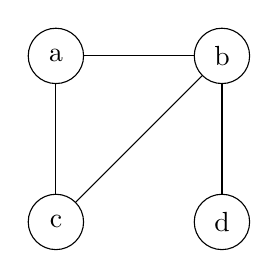
\begin{tikzpicture}
        \tikzstyle{every node}=[draw,circle,minimum size = 2em,node distance = 6em]
        \node (a) {a};
        \node [right of = a] (b) {b} edge(a);
        \node [below of = a] (c) {c} edge(a) edge(b);
        \node [below of = b] {d} edge(b);
    \end{tikzpicture}
\end{figure}

The adjacency matrix and adjacency list for \cref{example_graph} would be:
\begin{table}[ht!]
\begin{minipage}[b]{0.56\linewidth}
\centering
    \begin{tabular}{l|llll}
        & A & B & C & D \\ \hline
         A & 0  & 1  & 1  & 0  \\
         B & 1  & 0  & 1  & 1  \\
         C & 1  & 1  & 0  & 0  \\
         D & 0  & 1  & 0  & 0  \\
    \end{tabular}
    \caption{Adjacency Matrix}
    \label{table:student}
\end{minipage}\hfill
\begin{minipage}[b]{0.4\linewidth}
\centering
\begin{tikzpicture}
    \matrix (M) [matrix of nodes,
                column sep=-\pgflinewidth,
                row sep=0pt,
                nodes in empty cells,
                nodes={draw,fill=gray!20,minimum width=.5cm,outer sep=0pt,minimum height=.7cm,anchor=center},
                column 1/.style={minimum height=.8cm, minimum width=2em}]{
        a &[8mm] b & \mbox{} &[4mm] c & /       \\
        b & a      & \mbox{} & c      & \mbox{}  & [4mm]d    & /  \\
        c & a      & \mbox{} & b      & /         \\
        d & b      & \mbox{} & /      & \mbox{}  \\
    };
    \foreach \i in {1,2,3,4}{
        \path (M-\i-1) [late options={label=left:\i}];
        \draw[->] (M-\i-1.east)--(M-\i-2.west);
        \draw[->] (M-\i-3.center)--(M-\i-4.west);
    }
    \draw[->] (M-2-5.center)--(M-2-6.west);
\end{tikzpicture}
\captionof{figure}{Adjacency List}
\label{fig:image}
\end{minipage}
\end{table}

The running time for these two data structures are shown in
\cref{table:running_time_of_amaj}.

\begin{table}[H]
    \caption{Running Time Analysis for Adjacency Matrix and Adjacency List}
    \label{table:running_time_of_amaj}
    \centering
    \begin{tabular}{l|c|c}
        \hline
        Time & Adjacency Matrix & Adjacency List \\\hline
        visit neighbor & \bigO{1} & \bigO{1}\\
        visit all neighbors & \bigO{n} & \bigO{degree(v)} \\
        test if $uv \in E$ & \bigO{1} & \tikzmark{runanaadaj1}{\bigO{degree(v)}}\\
        add/delete edge & \bigO{1} & \tikzmark{runanaadaj2}{\bigO{n}}\\
        size & \bigO{mn} & \bigO{m+n}
    \end{tabular}
    \begin{tikzpicture}[remember picture,overlay,node distance = 1cm]
        \node[below right = 4em and 1em of runanaadaj1] (notes) {\bigO{1} with hashing.};
        \draw[->,thick] (runanaadaj1.east) to [in=90,out=0] (notes.north);
        \draw[->,thick] (runanaadaj2.east) to [in=90,out=0] (notes.north);
    \end{tikzpicture}
\end{table}



% \pagebreak

% \section{NP-Hardness}

\subsection{A Game You Can't Win}
Given a box with $n$ binary switches and a light bulb.
Inside the box is a boolean circuit, s.t
\begin{itemize}
    \item \textsc{And}, \textsc{Or}, \textsc{Not} gates, as shown in \cref{fig:gates};
    \item $n$ input wires, one per switch;
    \item Gates connected to single output, i.e the light bulb.
\end{itemize}
\begin{figure}[H]
    \centering
    \includegraphics{fig/gates}
    \caption{An \textsc{And}, an \textsc{Or}, and a \textsc{Not} gate}
    \label{fig:gates}
\end{figure}
An example is shown in \cref{fig:lightbulb}
\begin{figure}[H]
    \centering
    \includegraphics[scale=1.5]{fig/lightbulb}
    \caption{A boolean circuit}
    \label{fig:lightbulb}
\end{figure}
We want to know if there is a way to set switches s.t
light bulb turns on.
There are $2^n$ possible binary inputs. There is an \bigO{n} size circuit
which accepts a single strings and rejects all others.
Hence, if you cannot see inside, in worst case you must try all $2^n$ strings.

Suppose now you can see inside box. Can you do better than guessing all strings?
The answer is nobody knows for sure but many believe not.

The problem of determining if boolean circuit has satisfying assignment is all
\textsc{CircuitSAT}.

\subsection{P versus NP}
Minimum for an algorithm to be efficient is that it runs in polynomial time,
i.e \bigO{n^c} for constant $c$, $n$ is input size.
In this course, we focused on problems with polynomial solutions where $c$ is small.
\begin{itemize}
    \item Some problems known to require exponential time, i.e \bigO{c^n}, $c>1$.
    \item Some problems cannot even be solved (for example, Halting Problem).
    \item Some problems we don't know how hard.
\end{itemize}
NP-hard is a class most believe cannot be solved in polynomial time,
but no one knows for sure.

A decision problem is a problem whose output is a single boolean value,
i.e. \textsc{Yes/No}.
For example: LIS was an optimization problem. $\rightarrow$ ``Is there any increasing sequence of length $\geq k$?''
is a decision problem.
\begin{itemize}[leftmargin=.75in]
    \item[P] Set of decision solvable in polynomial time, i.e ``efficiently solvable''.
    \item[NP] Decision problems s.t if answer in \textsc{Yes}, then there is a proof
        that can be checked in polynomial time. $\rightarrow$ can verify \textsc{Yes} if proof given to us.
    \item[Co-NP] Decision problems s.t if answer in \textsc{No}, then there is a proof
        that can be checked in polynomial time. $\rightarrow$ can verify \textsc{No} if proof given to us.
\end{itemize}
\textsc{CircuitSAT} is in NP, if satisfying string, then given string, it is easy to verify.

Why do most believe $P \neq NP$?
One intuition is that: solving problems is harder than verifying solutions.
\begin{itemize}[leftmargin=.75in]
    \item[P] Problem in CLRS that you can solve quickly.
    \item[NP] Problem in CLRS that you can verify solution quickly.
\end{itemize}

\subsection{NP-Hard/NP-Complete}
A problem $\Pi$ is NP-hard if a polynomial time algorithm for $\Pi$ implies
polynomial time algorithm for all problems in NP.
\begin{quote}
    $\Pi$ is NP-hard $\leftrightarrow$ If $\Pi$ solution in polynomial time, then P = NP.
\end{quote}

Hence, most believe no NP-hard problem solvable in polynomial time.

$\Pi$ is NP-complete if $\Pi$ is NP-hard and $\Pi \in \text{NP}$.

Thousands of problems have been shown to be NPC.
How does one prove something NP-hard or NPC?

\begin{theorem}[Cook-Levin Theorem] \textsc{CircuitSAT} is NPC.\end{theorem}

All problems that are shown to be NPC, reduce from \textsc{CircuitSAT}.

\subsection{Reductions \& SAT}
To prove any problem other than the \textsc{CircuitSAT} is NP-hard, use reduction.
Reducing problem A to problem B means solving A using solution for B.
To prove B is NP-hard, reduce \underline{from} known NP-hard problem A \underline{to} problem B.
Require reduction to be polynomial time in the A instance size.

Intuition: we are sure A is hard, Hence B must be hard, since otherwise it implies A can be
solved quickly.

Often write: $B \geq_p A$,
$\geq_p$ stands for B at least as hard as A ignoring polynomial factor.

A may still require more time to solve bu not more than polynomial factor.

Given a boolean formula, is there a satisfying assignment,
i.e a binary assignment variables evaluating to be true.
For example: 
\[(a \lor b \lor c \lor \overline{d}) \Longleftrightarrow ((b \land \overline{c}) \lor \overline{(\overline{a} \Rightarrow d)} \lor (c \neq a \land b))\]
To prove SAT is NP-hard, we reduce from \textsc{CircuitSAT}.
So given a boolean circuit (i.e. a DAG), we must convert to an equivalent boolean formula.

One solution: circuit has single output gate,
so start at root gate, recursively write formula,
for each subtree and combine formula with root gate operation.
This method takes exponential time since DAG, not a tree.

Here is the polynomial time reduction:
\begin{enumerate}
    \item For each gate output wire create a variable: $y_1 \ldots y_n$ as gates outputs,
        $x_1 \ldots x_m$ as circuit input, $z$ as circuit output.
    \item For each gate wire clause saying inputs match output.
    \item Take \textsc{And} of all these clauses and $z$.
    \item This says all gates work properly and output is $1$.
\end{enumerate}
For example, \cref{fig:sat} shows the formula transformed from \cref{fig:lightbulb}.
\begin{figure}[H]
    \centering
    \includegraphics[scale=1.25]{fig/sat}
\begin{align*}
    (y_1 = x_1 \land x_4)\land&(y_2 = \overline{x_4})\land(y_3 = x_3 \land y_2)\land(y_4 = y_1 \land x_2)\land\\
    &(y_5 = \overline{x_2})\land(y_6 = \overline{x_5})\land(y_7 = y3 \lor y_5)\land(z = y_4 \land y_7 \land y_6) \land z
\end{align*}
    \caption{A boolean circuit with gate variables added, and an equivalent boolean formula}
    \label{fig:sat}
\end{figure}
The original circuit is satisfiable if and only if the boolean formula is.
\begin{itemize}[leftmargin=.75in]
    \item[$\Longrightarrow$] Given satisfying assignment to circuit, can find satisfying assignment to formula
        by computing output of every gate.
    \item[$\Longleftarrow$] Given satisfying assignment to formula, just ignore $y_i$s and $z$ to get circuit input.
\end{itemize}
By this, we can produce formula from circuit in linear time.
Thus, polynomial time reduction from \textsc{CircuitSAT} to SAT.

\subsection{3SAT}
Boolean formula is in conjunctive normal form (CNF) if it is the
conjunction (\textsc{And}) of clause,
each of which is a disjunction (\textsc{Or}) of literals,
each of which is a variable of its negation.

A 3CNF formula is a CNF formula with exactly 3 literals per clause.

\begin{theorem}
    3SAT is NP-complete.
\end{theorem}
\begin{proof}
To prove 3SAT $\in$ NP, given satisfying assignment, plug in values and evaluate.

To prove 3SAT is NP-hard: (reduce from \textsc{CircuitSAT})

Given \textsc{CircuitSAT} instance, convert to 3SAT instance:
Assume each gate has fan in at most 2.
\begin{enumerate}
    \item Write circuit as formula with one clause per gate;
    \item Change each gate clause to CNF:
        \begin{align*}
            a=b \land c &\Longleftrightarrow (a \lor \overline{b} \lor \overline{c}) \land
                (\overline{a} \lor b) \land (\overline{a} \lor c) \\
            a=b \lor c &\Longleftrightarrow (\overline{a} \lor b \lor c) \land
                (a \lor \overline{b}) \land (a \lor \overline{c}) \\
            a = \overline{b} &\Longleftrightarrow (a \lor b) \land (\overline{a} \lor \overline{b})
        \end{align*}
    \item Convert to 3CNF (exactly 3 literals per clause)
        \begin{align*}
            a &\Longleftrightarrow (a \lor x \lor y) \land (a \lor \overline{x} \lor y) \land
                (a \lor x \lor \overline{y}) \land (a \lor \overline{x} \lor \overline{y}) \\
            a \lor b &\Longleftrightarrow (a \lor b \lor x) \land (a \lor b \lor \overline{x})
        \end{align*}
\end{enumerate}
Polynomial time reduction, hence 3SAT is NP-hard.
\end{proof}

\subsection{Independent Set}
Let $G$ be an undirected graph. An independent set in $G$ is a set of vertices
with no edge between them.

\noindent\textbf{Independent Set Problem}: Given $G$ and integer $k$, is there an independent set of size $\geq k$.

\noindent\textbf{Max Independent Set Problem}: Given $G$, find the size of largest independent set.

\begin{proof}
We prove the Independent Set Problem is NP-hard by reducing from 3SAT:
Input is a 3SAT instance with $x$ clauses.
For each literal of each clause, create a vertex.
Add an edge between two vertices if either:
\begin{itemize}
    \item literals are in the same clause;
    \item literal correspond to variable and its negation.
\end{itemize}
For example the following formula
\[(a \lor b \lor c) \land (b \lor \overline{c} \lor \overline{d}) \land
    (\overline{a} \lor c \lor d) \land (a \lor \overline{b} \lor \overline{d})\]
is transformed into the following graph:

\begin{figure}[H]
    \centering
    \includegraphics[scale=1.5]{fig/indepset}
    \caption{A graph derived from a 3CNF, and an independent set of size 4}
    \label{fig:indepset}
\end{figure}

The formula is satisfiable if and only if independent set of size $x$:
\begin{itemize}[leftmargin=.75in]
    \item[$\Longrightarrow$] To get satisfying assignment, set each literal from
        independent set to be true.\\
        Since contradictory literals connected by edge, this assignment consistent.\\
        The formula is evaluated to be true since each clause satisfied.
    \item[$\Longleftarrow$] If there is a satisfying assignment, choose one literal for
        each clause that is true.\\
        These literal are independent set in graph since from different clauses and consistent.
\end{itemize}

This proves \textsc{IndepSet}(G,K) is NP-hard.

Since given a subset, can easily check if it is independent set and size $\geq k$,
\textsc{IndepSet}(G,K) $\in$ NP.

Hence, \textsc{IndepSet} in NP-complete.
\end{proof}

\subsection{Clique}
A clique is a subset of vertices where every pair connected.
MaxClique asks for size of largest clique.

\textsc{Clique} is NPC.

Define complement graph $\overline{G}$ as a vertex set, where edge is in $\overline{G}$ if and only if
the edge is not in $G$.
A set if vertices is independent set of $G$ if and only if the same set of vertices is clique in $\overline{G}$.

\subsection{Vertex Cover}
A vertex cover is a set of vertices such that every edge in $G$ is adjacent to vertex in set.
Minimum vertex cover asks for size of smallest vertex cover.
\textsc{VertexCover} asks if vertex cover of size $\leq k$.

\begin{claim}
    A set $I \subseteq V$ is independent set if and only if $V \setminus I$ is the vertex cover.
\end{claim}

\begin{itemize}[leftmargin=.75in]
    \item[$\Longrightarrow$] Consider edge $uv$, cannot have both $u$ and $v \in I$,
        so at least one endpoint in $V \setminus I$.
    \item[$\Longleftarrow$] If $i$ is not independent set, then for some edge $uv$,
        $u,v \in I$, hence $uv$ not covered in $V \setminus I$, (not vertex cover).
\end{itemize}

Hence, \textsc{IndepSet} of size $\geq k$ if and only if vertex cover of size $\leq n-k$.
$I_{max}$ independent set if and only $V \setminus I$ is minimum vertex cover.

\subsection{Some Intuition}
The reduction tree of the problems discussed in the note and homework is shown in \cref{fig:redtree}.

\begin{figure}[H]
    \caption{Reduction Tree}\label{fig:redtree}
    \centering
    \begin{tikzpicture}[every tree node/.style={draw=none},level distance = 1.5cm]
        \Tree [.\textsc{CircuitSAT}
            [.SAT ]
            [.3SAT
                [.\textsc{IndepSet}
                    [.\textsc{Clique} ]
                    [.\textsc{VertexCover}
                        [.\textsc{HittingSet} ]
                    ]
                ]
            ]
        ]
    \end{tikzpicture}
\end{figure}

Here are some other NPC problems:
\begin{itemize}
    \item 3 Coloring
    \item Hamiltonian Path/Cycle
    \item If weighted, TS
\end{itemize}

And here are some Polynomial time problem:
\begin{itemize}
    \item Edge Cover
    \item 2SAT
    \item 2 Coloring
    \item Euler tour in connected even degree vertex graph.
\end{itemize}

And here is the end of the lecture note.


\end{document}
